% !TEX root = ../main.tex

\chapter{Application on historical dataset}
\label{chap:Application on historical dataset}

For purpose of demonstrating for demand I'm using data from US electricity consumption~\autocite{us-elec} It offers per month aggregation of electrical energy used per state, and for purpose of illustration I'm using whole US aggregated. Data ranges from 1990 till February 2016. I'm using restricted version from 1990 till 2005 aggregated on yearly basis. Full data plot is in figure~\ref{fig:supply}

\begin{figure}[]
  \centering
  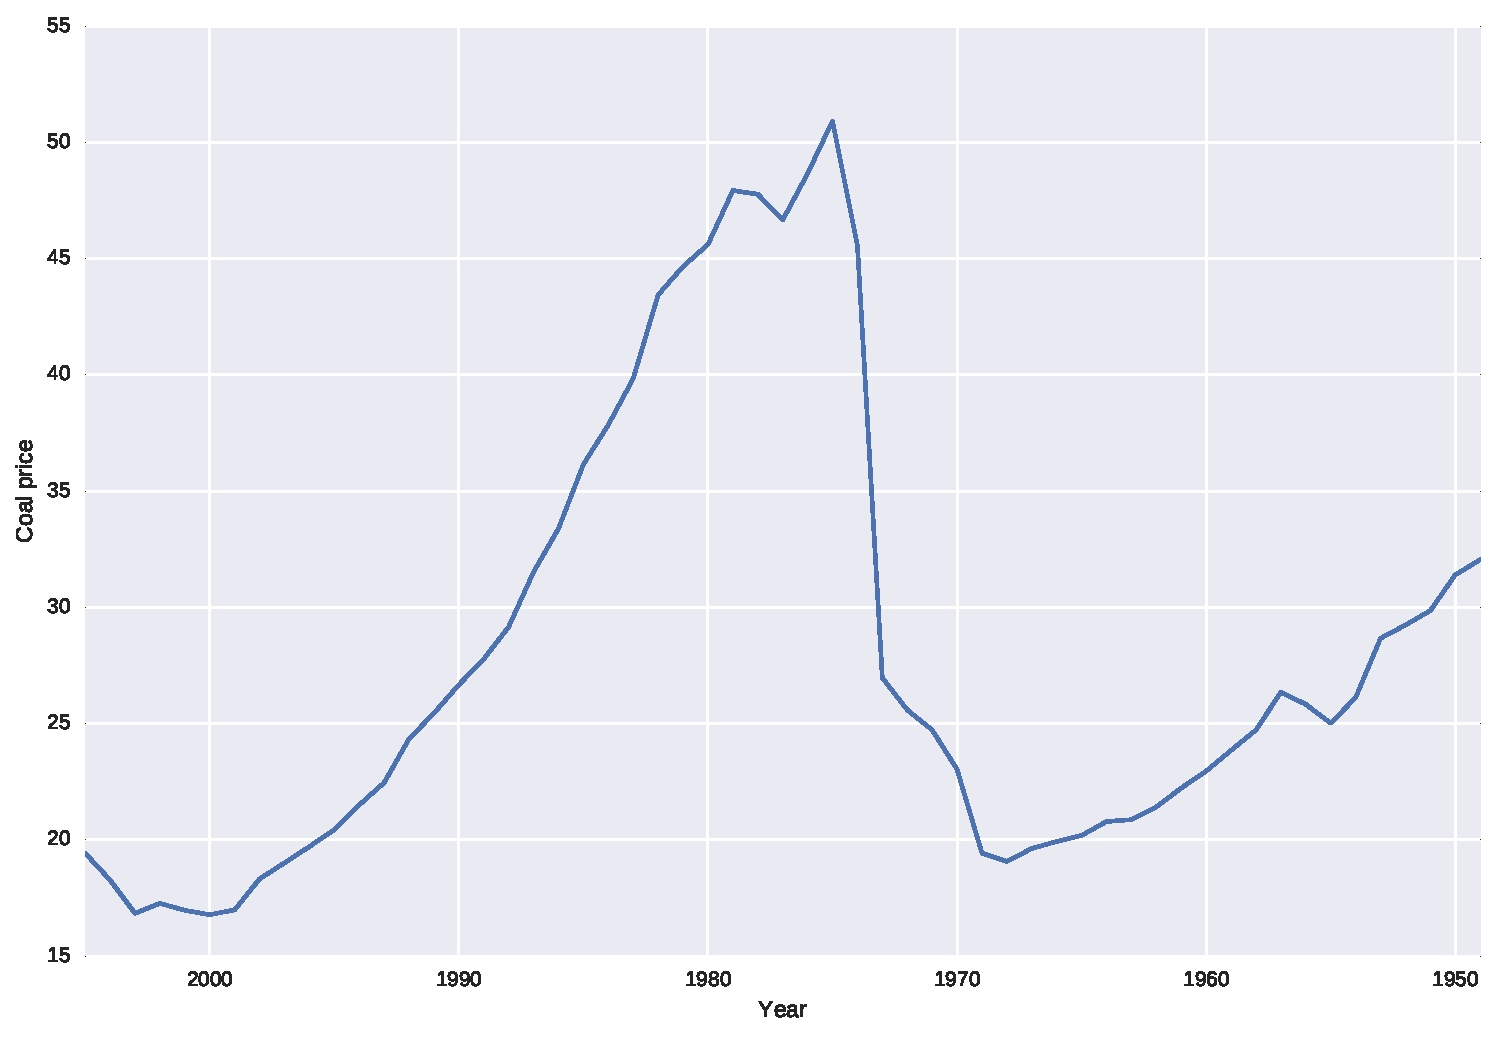
\includegraphics[width=0.8\linewidth]{supply}
  \caption{Yearly coal prices. Green are prediction with ARIMA(0,1,1) model}
  \label{fig:supply}
\end{figure}

For supply unit cost, for illustrative purposes I'm using historic American coal price~\autocite{us-coal}. It is yearly based from 1950 till 2005. The data is plot is in figure~\ref{fig:demand}.

For purposes of this analysis, data from 2000 till 2005 is going to be unknown and serve as demonstration of programming support helper functions. Whole programming support can be found at URL~\autocite{code}. Forecasting is done by fitting ARIMA model, where model selection is done with lowest Akaike information criterion~\autocite{Akaike1974}.

\begin{figure}[]
  \centering
  \includegraphics[width=0.8\linewidth]{demand}
  \caption{Yearly electricity demand. Green are predictions with ARIMA(1,2,0) model}
  \label{fig:demand}
\end{figure}

As we can see from figures~\ref{fig:demand} and~\ref{fig:supply}, automatic data forecasting yields subpar performance compared to true future data in both supply cost and in demand quantity time series. In supply it predicts decline in price, while the price is increasing, and in demand quantity it underestimates increase in demand.

Which is partially to be expected given model has only time series data as input, without all other world parameters influencing demand quantity and supply cost. For such cases expert opinions is of utmost importance and decision maker should decide which forecasted quantities make sense and which ones are underestimated/overestimated. Automatic approach works only for the most simplest cases, and knowledge of dedicated system or libraries would enable decision maker greater agility in implementing models, finding solutions and its refinement.

Despite mentioned shortcomings in this particular dataset, automatic method with backlogging cost $b=100$ and holding cost $h=1$, achieves 0.02\% accuracy for first step procurement quantity compared to ideal solution. Detailed jupyter notebook is located at URL~\autocite{jup}.
